\documentclass[border=10pt]{standalone}

\usepackage{tikz}
\usetikzlibrary{arrows.meta,decorations.pathreplacing,patterns}
\usepackage{amsmath}

\begin{document}
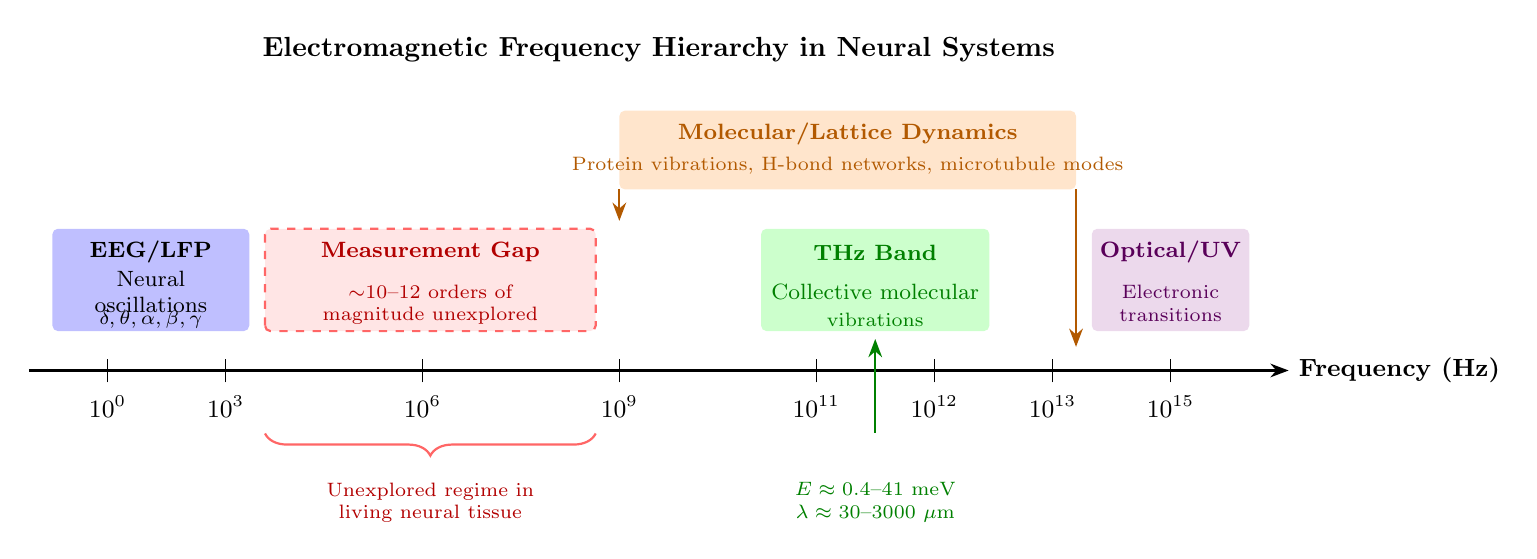
\begin{tikzpicture}[>=Stealth, font=\small]

% Main axis
\draw[->, thick] (0,0) -- (16,0) node[right] {\textbf{Frequency (Hz)}};

% Frequency labels along axis
\foreach \x/\lab in {1/$10^{0}$, 2.5/$10^{3}$, 5/$10^{6}$, 7.5/$10^{9}$, 10/$10^{11}$, 11.5/$10^{12}$, 13/$10^{13}$, 14.5/$10^{15}$} {
  \draw (\x, -0.15) -- (\x, 0.15);
  \node[below] at (\x, -0.2) {\lab};
}

% EEG accessible range
\fill[blue!25, rounded corners=2pt] (0.3, 0.5) rectangle (2.8, 1.8);
\node[align=center, font=\footnotesize\bfseries] at (1.55, 1.5) {EEG/LFP};
\node[align=center, font=\footnotesize] at (1.55, 1.0) {Neural\\oscillations};
\node[align=center, font=\scriptsize] at (1.55, 0.65) {$\delta, \theta, \alpha, \beta, \gamma$};

% Measurement gap
\fill[red!10, rounded corners=2pt] (3.0, 0.5) rectangle (7.2, 1.8);
\draw[red!60, thick, dashed, rounded corners=2pt] (3.0, 0.5) rectangle (7.2, 1.8);
\node[align=center, font=\footnotesize\bfseries, red!70!black] at (5.1, 1.5) {Measurement Gap};
\node[align=center, font=\scriptsize, red!70!black] at (5.1, 1.0) {$\sim$10--12 orders of};
\node[align=center, font=\scriptsize, red!70!black] at (5.1, 0.7) {magnitude unexplored};

% THz regime
\fill[green!20, rounded corners=2pt] (9.3, 0.5) rectangle (12.2, 1.8);
\node[align=center, font=\footnotesize\bfseries, green!50!black] at (10.75, 1.5) {THz Band};
\node[align=center, font=\footnotesize, green!50!black] at (10.75, 1.0) {Collective molecular};
\node[align=center, font=\scriptsize, green!50!black] at (10.75, 0.65) {vibrations};

% Molecular dynamics range
\fill[orange!20, rounded corners=2pt] (7.5, 2.3) rectangle (13.3, 3.3);
\node[align=center, font=\footnotesize\bfseries, orange!70!black] at (10.4, 3.0) {Molecular/Lattice Dynamics};
\node[align=center, font=\scriptsize, orange!70!black] at (10.4, 2.6) {Protein vibrations, H-bond networks, microtubule modes};

% Arrows connecting
\draw[->, thick, orange!70!black] (7.5, 2.3) -- (7.5, 1.9);
\draw[->, thick, orange!70!black] (13.3, 2.3) -- (13.3, 0.3);

% Brace for gap
\draw[decorate, decoration={brace, amplitude=8pt, mirror}, thick, red!60] (3.0, -0.8) -- (7.2, -0.8);
\node[below, font=\scriptsize, red!70!black, align=center] at (5.1, -1.3) {Unexplored regime in\\living neural tissue};

% Energy scale annotation for THz
\draw[<-, thick, green!50!black] (10.75, 0.4) -- (10.75, -0.8);
\node[below, font=\scriptsize, green!50!black, align=center] at (10.75, -1.3) {$E \approx 0.4$--$41$~meV\\$\lambda \approx 30$--$3000~\mu$m};

% Optical/UV range
\fill[violet!15, rounded corners=2pt] (13.5, 0.5) rectangle (15.5, 1.8);
\node[align=center, font=\footnotesize\bfseries, violet!70!black] at (14.5, 1.5) {Optical/UV};
\node[align=center, font=\scriptsize, violet!70!black] at (14.5, 1.0) {Electronic};
\node[align=center, font=\scriptsize, violet!70!black] at (14.5, 0.7) {transitions};

% Title
\node[above, font=\normalsize\bfseries] at (8, 3.8) {Electromagnetic Frequency Hierarchy in Neural Systems};

\end{tikzpicture}
\end{document}
